Au départ nous étions parti sur une architecture avec un serveur web qui communiquait avec les clients grâce à des requêtes web HTTP.

Malheureusement cette architecture n'était pas adaptée pour un jeu de ce type puisque au moment où un joueur joue un coup, l'autre joueur doit être notifié de ce changement. Or si on utilise un serveur web HTTP le client devrait faire une requête au serveur pour être mis au courant, ce qui n'est pas pratique.

Pour un changement en direct sans faire une boucle de requêtes continuelles, il faudrait un système où le serveur peut envoyer un message au client sans requête au préalable.

C'est pour cela qu'une architecture avec des web sockets a été la solution que nous avons choisie.
Cette architecture permet d'envoyer des messages ou des données aux clients sans requête préalable.


\begin{figure}[H]
    \centering
    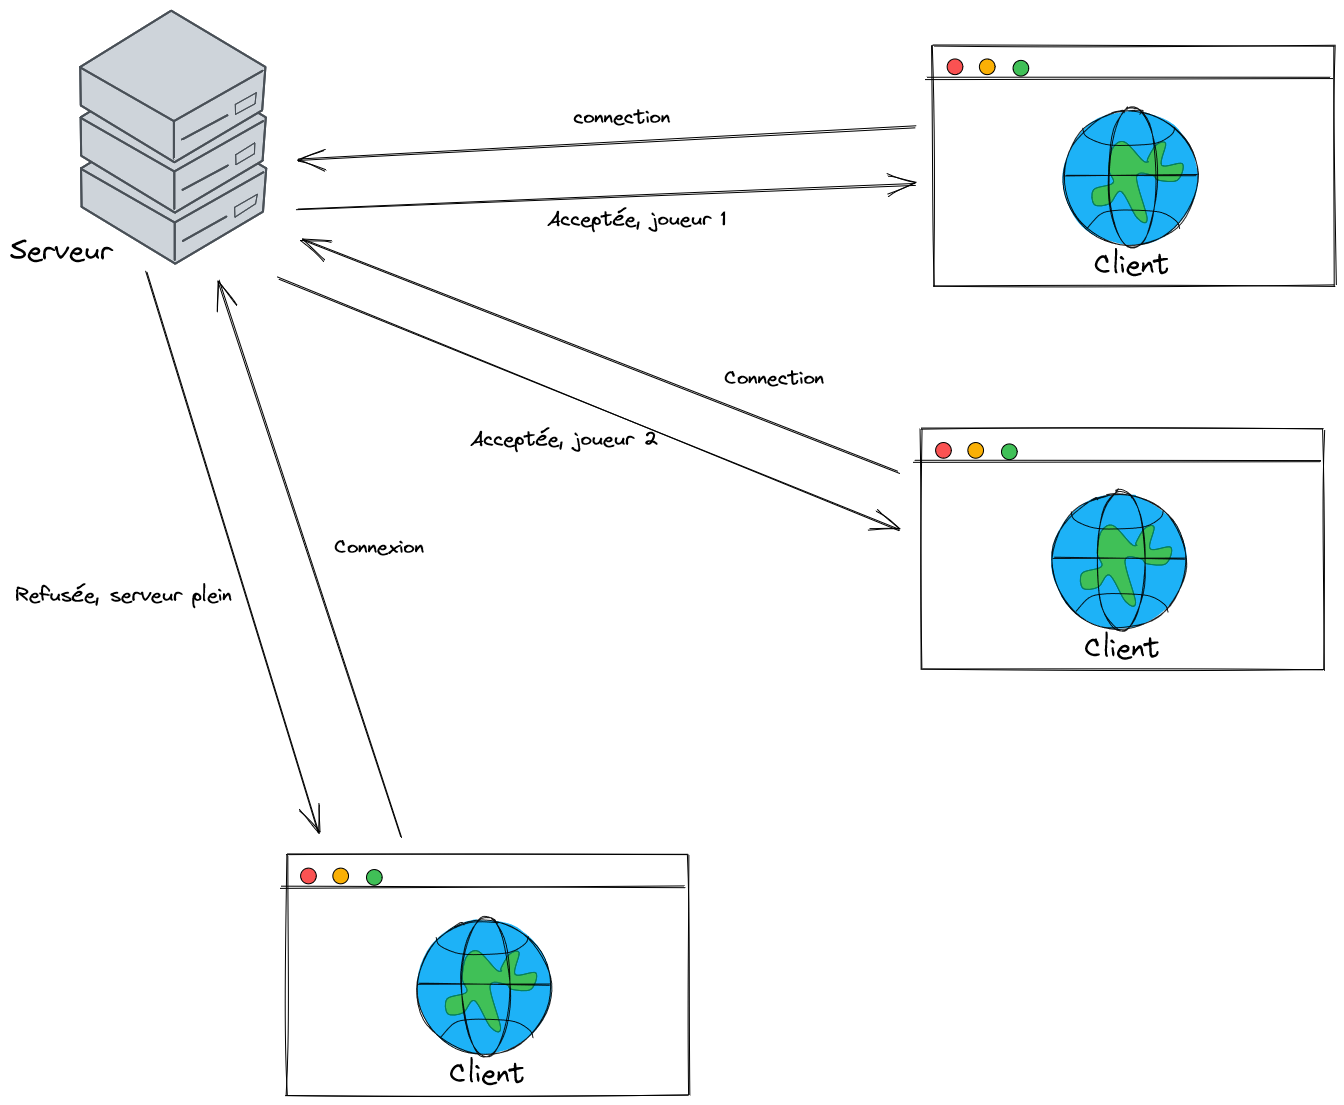
\includegraphics[scale=0.25]{data/reseau_initialisation.png}
    \caption{Phase de connexion des joueurs au serveur}
\end{figure}

Ici on peut voir la première phase du serveur qui permet d'enregistrer les connexions des deux joueurs pour créer une partie.

La partie de connexion est gérée par la bibliothèque {\tt socket-io} que nous utilisons pour le serveur et le client. C'est l'avantage essentiel d'utiliser la même technologie sur le backend et le frontend.

Dans le serveur, nous sauvegardons les sockets qui se connectent au serveur. La limite est de 2 puisqu'il y a 2 joueurs maximum. Quand les 2 joueurs sont bien connectés, la partie est pleine. S'il y en a déjà 2 lors d'une connexion d'un troisième socket, alors la connexion de la troisième est refusée et cette dernière reçoit un code d'erreur, {\tt full}, que le frontend de ce socket va afficher à l'utilisateur.
Si un autre joueur essaie de se connecter, alors le socket n'est pas sauvegardé dans le serveur et elle est déconnectée, il reçoit également une erreur, {\tt full}, qui va s'afficher dans le terminal.

Une fois les deux joueurs créés et la partie initialisée, la carte est envoyée aux deux joueurs pour l'affichage. Voir ci-dessous \ref{reseau_carte}.

\begin{figure}[H]
    \centering
    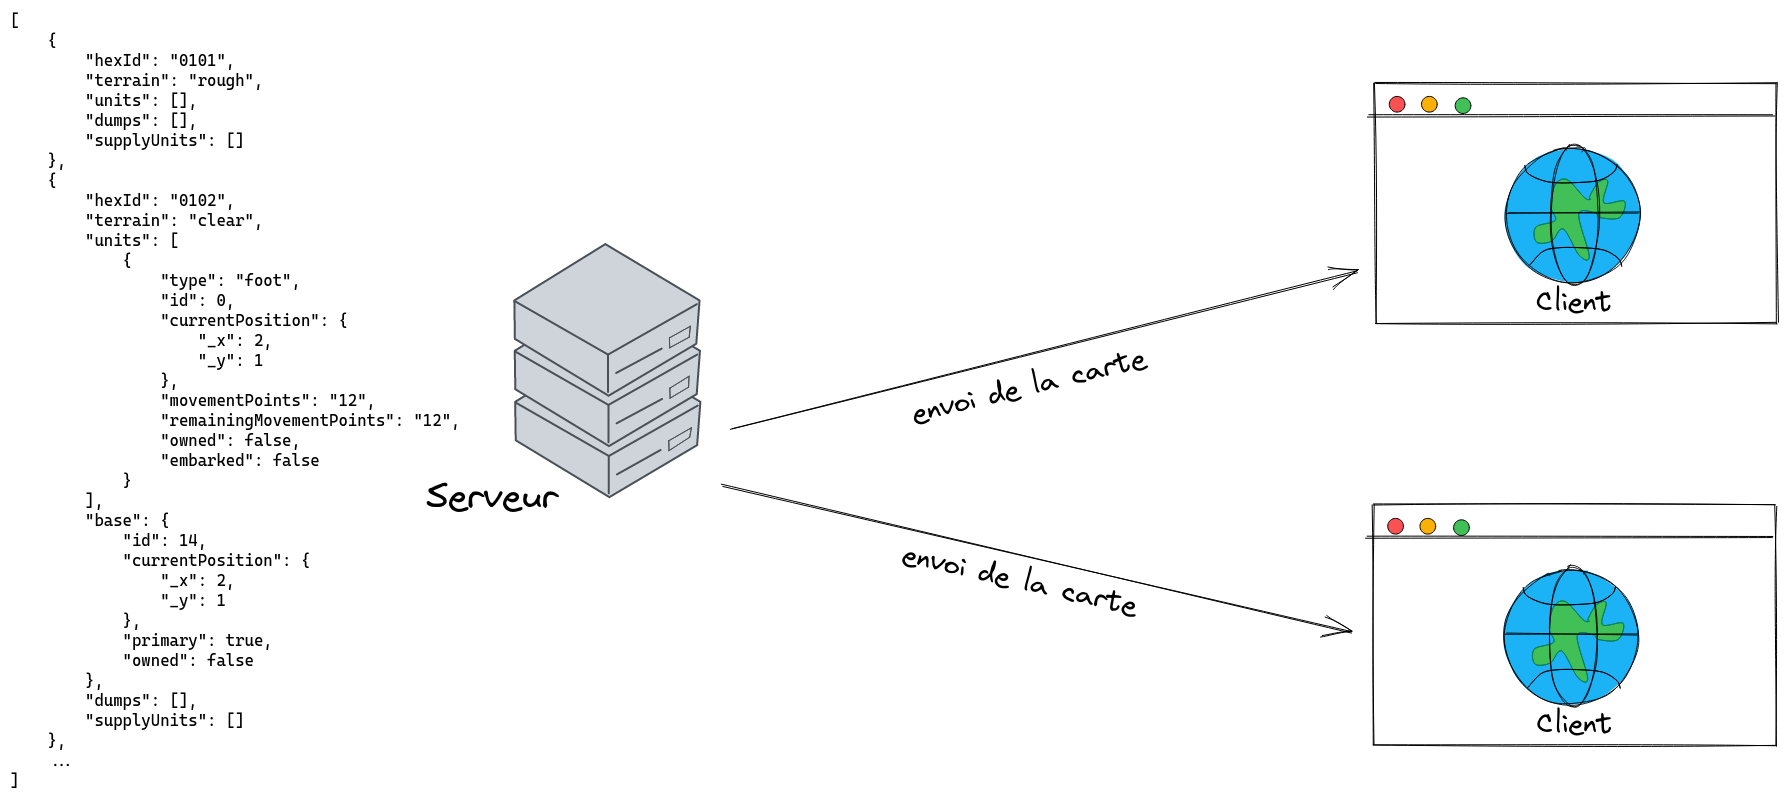
\includegraphics[scale=0.25]{data/reseau_map.png}
    \caption{Phase d'envoi de la carte aux joueurs}
    \label{reseau_carte}
\end{figure}

Le code à gauche du serveur est le début du {\tt JSON} original envoyé à chaque client.
On peut voir comment il est constitué : c'est un tableau d'objets. Chacun de ces objets représente une case.
Chaque case possède un {\tt id}, ici appelé {\tt hexId}, un identifiant, ainsi qu'un {\tt terrain} qui décrit son type de terrain.
Il possède aussi 3 aux champs, {\tt units}, {\tt dumps} et {\tt supplyUnits} qui sont des tableaux d'objets.
Comme leurs noms l'indique ces objets représentent des tableaux d'unités, de dépôts ou d'unités de ravitaillement.

À partir de ce moment-là, le moteur graphique du jeu est chargé de dessiner la carte reçue en JSON.
L'action \ref{reseau_carte} se répète à chaque changement de la carte dans le jeu.


\begin{figure}[H]
    \centering
    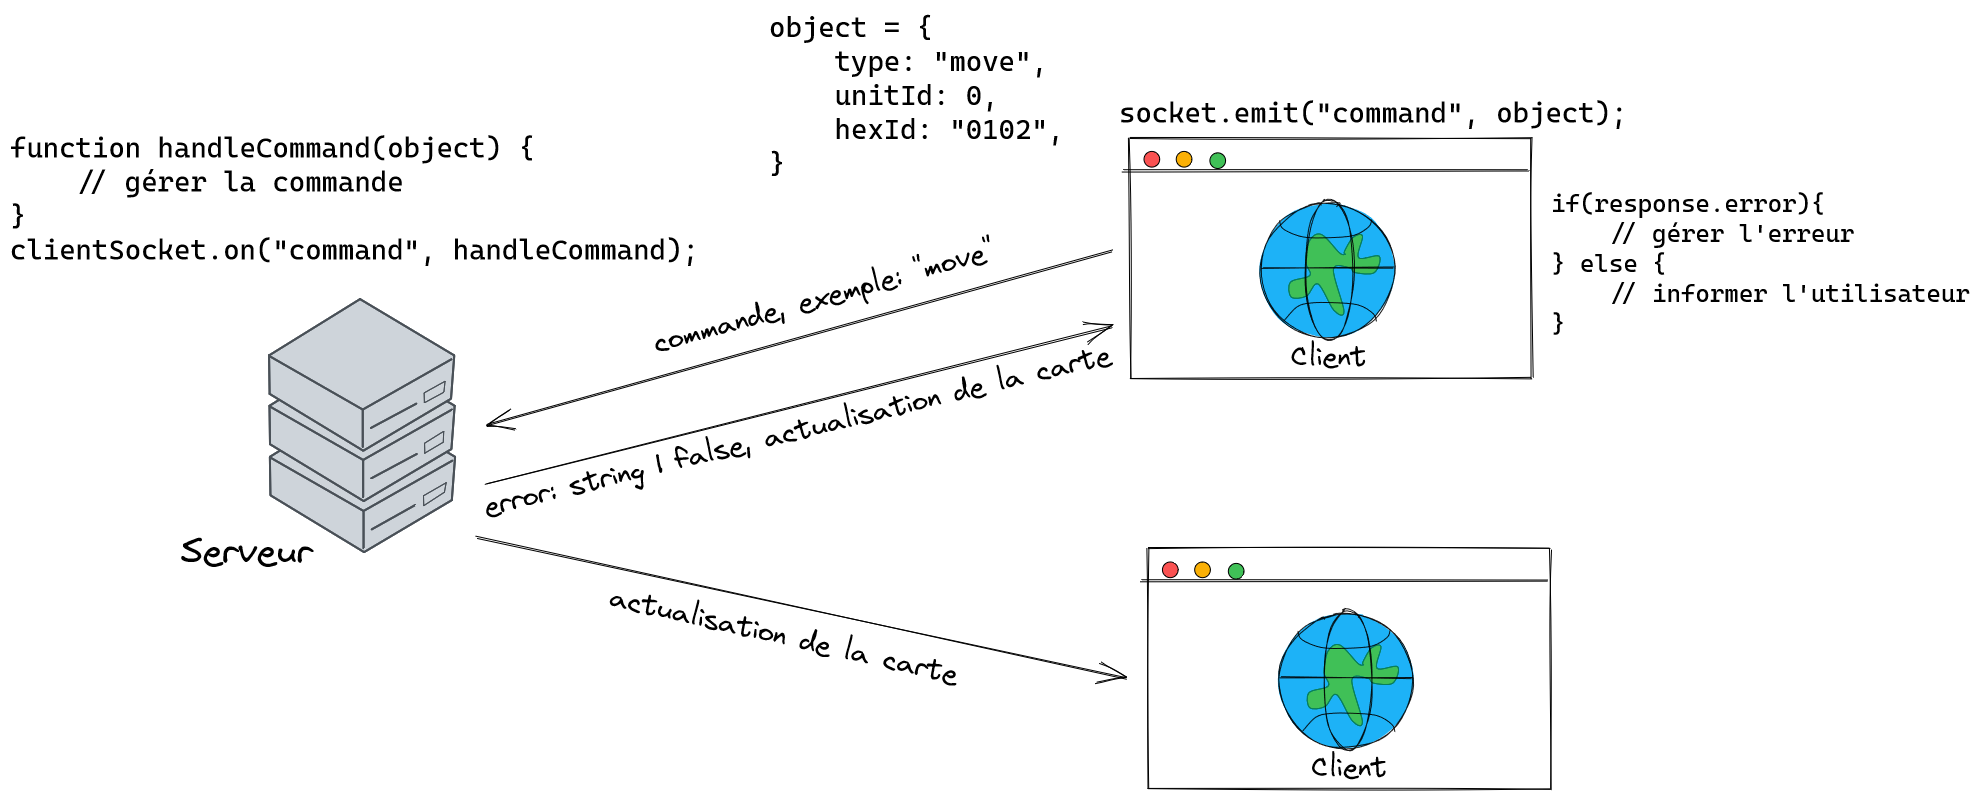
\includegraphics[scale=0.25]{data/reseau_commande.png}
    \caption{Phase de jeu, exemple de commande {\tt move}}
    \label{reseau_commande}
\end{figure}

La figure \ref{reseau_commande} ci-dessus est un exemple de commande envoyée par le client.
Ici, le joueur souhaite bouger l'unité d'identifiant {\tt 0} de son hexagone vers l'hexagone {\tt 0102}.

Dans le client en haut à droite, on peut voir que la {\tt socket} utilisée par le joueur pour communiquer au serveur
envoie l'événement {\tt command} au serveur. En paramètre de cet événement, le client joint un objet qui va contenir les
paramètres de la commande. Ces paramètres sont décrits dans l'objet {\tt object}. On peut y voir 3 champs.

Le premier champ {\tt type} indique le type de la commande. Ici, on peut voir que le client indique le type {\tt move}.
Les autres champs dépendent du type de la commande. Pour le type {\tt move}, il faut indiquer l'identifiant de l'unité et
l'identifiant de l'hexagone de destination.
Chacun de ces paramètres sont décrits dans l'objet. {\tt unitId} décrit l'identifiant de l'unité, {\tt hexId} décrit l'identifiant
de l'hexagone de destination.

Cet objet est donc envoyé au serveur qui va le recevoir grâce à sa {\tt socket} reliée à celle du client.
Celle ci reçoit directement l'objet {\tt object} envoyé et va le traiter.
Ce traitement a deux étapes :
\begin{enumerate}
    \item On vérifie que les paramètres de la requête sont corrects. Ici, on va vérifier que les numéros sont corrects
          et qu'ils décrivent bien une unité existante que le joueur possède et un hexagone valide.
    \item On effectue la commande. La commande elle-même va vérifier que l'unité en question possède assez de points de mouvements et l'hexagone de destination est vide ou allié.
\end{enumerate}


Si une erreur est provoquée soit par la phase de vérification ou par la phase de commande, le serveur envoie un objet contenant le champ {\tt error} qui contient le code d'erreur.
Ce code d'erreur est ensuite reçu par le client qui va l'interpréter à l'utilisateur.

Si la commande est valide et effectue un changement de la carte, le serveur envoie la nouvelle carte aux deux joueurs.
